\begin{definition}
    \textbf{Spacerem losowym} na nieskierowanym grafie \( G \) nazywamy łańcuch Markowa, którego stany odpowiadają wierzchołkom grafu. Prawdopodobieństwo przejścia ze stanu \( v \) do stanu \( u \) wynosi \( \frac{1}{\text{deg}(v)} \) gdy \( (v, u) \in \mathbb{E}\) i 0 w przeciwnym przypadku.
\end{definition}

\begin{theorem}[Lemat 7.12 P\&C] Spacer losowy na grafie \( G \) jest nieokresowy wtedy i tylko wtedy gdy \( G \) nie jest dwudzielny
\end{theorem}
\begin{proof}
    \(\left( \implies \right) \) Jeśli \(G\) jest dwudzielny, to do każdego wierzchołka \(v\) można wrócić tylko po parzystej liczbie kroków, bo co krok zmieniamy stronę, po której jesteśmy.

    \(\left( \impliedby \right) \) W niedwudzielnym \(G\) musi istnieć nieparzysty cykl. Niech \(v\) leży na tym cyklu. Z jednej strony można wyjść do dowolnego sąsiada \(v\) i wrócić, co da \(p_{vv} \left( 2 \right) >0\), a z drugiej można przejść całym cyklem, czyli \(p_{vv} \left( 2k+1 \right) >0\). Zatem okres \(v\) (czyli całego spaceru) to \(1\).
\end{proof}

\begin{theorem}[Lemat 7.13 P\&C] Spacer losowy na spójnym, niedwudzielnym grafie \( G \) posiada rozkład stacjonarny \( \bar \pi \) w którym \( \pi_v = \frac{\Deg(v)}{2|E|} \)
\end{theorem}
\begin{proof}
    Pokażemy, że tak zadane \(\bar\pi\) faktycznie jest rozkładem stacjonarnym. Mamy
    \[ \sum_{v\in V \left( G  \right) }^{} \pi_v = \sum_{v\in V \left( G  \right) }^{} \frac{d \left( v  \right) }{2 \mathbb{E}\left( G  \right) } = \frac{1}{2 \mathbb{E}\left( G  \right)} \sum_{v\in V \left( G  \right) }^{} d \left( v  \right) = 1, \] 
    a więc faktycznie jest to rozkład. Mamy też
    \[ \left( \pi P \right)_v  = \sum_{u \in V \left( G  \right)}^{} \pi_u \cdot P_{uv} = \sum_{u \in N \left( v \right) }^{} \frac{d \left( u  \right) }{2 \mathbb{E}\left( G  \right) } \cdot \frac{1}{d \left( u \right) } = \frac{d \left( v  \right) }{2 \mathbb{E}\left( G  \right) } = \pi_v,\] 
    gdzie drugie przejście to zastosowanie określenia macierzy \(P\) dla spaceru.
\end{proof}

\begin{definition}
    Czas pokrycia grafu \(G\) to chwila (indeks łańcucha Markowa), w której spacer odwiedził już każdy wierzchołek. Taką zmienną losową oznaczamy \(C_G\).
\end{definition}

\begin{lemma}
    Dla każdej krawędzi \(uv\) w grafie \(G\) zachodzi \(\mathbb{E}\left[ r_{uv} \right] + \mathbb{E}\left[ r_{vu} \right] \le 2 \mathbb{E}\left( G  \right) \).
\end{lemma}
\begin{proof}
    Mając graf \(G\) będziemy tworzyć łańcuch Markowa na krawędziach skierowanych. Rozważamy skierowany graf \(D\), który jest grafem \(G\), w którym każda krawędź została przedstawiona jako dwie krawędzie skierowane. Stanem łańcucha będą krawędzie, a z zadanej krawędzi będzie można przejść do krawędzi wychodzących z jej końca (z równym prawdopodobieństwem).

    W takim łańcuchu rozkład jednostajny \(\pi_{uv} = \frac{1}{2 \mathbb{E}\left( G  \right) }\) jest stacjonarny. Po pierwsze \( \sum_{uv \in \mathbb{E}\left( D  \right) }^{} \pi_{uv} = \sum_{uv \in \mathbb{E}\left( D  \right) }^{} \frac{1}{2 \mathbb{E}\left( G  \right) } = 1\), więc jest to rozkład.
     Mamy też \[ \sum_{w\in N\left( u  \right) }^{} \pi_{wu} \frac{1}{d\left( u \right) } = \frac{1}{d\left( u  \right) }\cdot \frac{d\left( u  \right) }{2 \mathbb{E}\left( G  \right) } = \frac{1}{2\mathbb{E}\left( G  \right) } = \pi_{uv},\]
     gdzie \(uv\) jest pewną krawędzią w \(D\). Z tego wynika, że rozkład jest stacjonarny.

     Ograniczana wartość \(\mathbb{E}\left[ r_{uv} \right] + \mathbb{E}\left[ r_{vu} \right] \) jest oczekiwaną liczbą kroków w spacerze \(u \to v \to u \). W grafie \(D\) można patrzeć na spacer z krawędzi \(vu\) do \(vu\). Idzie on tak samo jak przejście z \(u\) do \(v\) i z powrotem do \(u\), ale ma ustaloną krawędź, którą trzeba wrócić do \(u\). Zatem będzie dłuższy od zwykłego spaceru po wierzchołkach i mamy 
     \[ \mathbb{E}\left[ r_{uv} \right] + \mathbb{E}\left[ r_{vu} \right] \le \mathbb{E}\left[ r_{(vu)(vu)} \right] = \frac{1}{\pi_{vu}} = 2\mathbb{E}\left( G  \right) . \] 
\end{proof}

\begin{theorem}[Twierdzenie 7.15 P\&C] Czas pokrycia grafu \( G = (V, E) \) jest ograniczony od góry przez \( 2|E|\left( |V|-1 \right)  \).
\end{theorem}
\begin{proof}
    Niech \(T\) będzie drzewem rozpinającym \(G\). Przejdziemy po jego wierzchołkach w kolejności DFSa. Niech \(v_0,v_1,\ldots,v_{2\left|V\right|-2}\) będą kolejnymi wierzchołkami odwiedzonymi przez DFSa. Oczekiwany czas pokrycia grafu jest ograniczony przez oczekiwany czas kolejnego odwiedzania wierzchołków wypisanych w takiej kolejności. Zatem 
    \[ \mathbb{E}\left[ C_G \right] \le \sum_{i=0}^{2\left|V\right|-3} \mathbb{E}\left[ r_{v_iv_{i+1}} \right] = \sum_{xy\in T}^{} \mathbb{E}\left[ r_{xy} \right] + \mathbb{E}\left[ r_{yx} \right] \le 2\left|\mathbb{E}\right|\cdot \left( \left|V\right|-1 \right)  .\] 
\end{proof}


\subsection{Ćwiczenia}

\begin{exercise}
    Mysz i kot niezależnie od siebie w sposób losowy biegają po spójnym, nieskierowanym, niedwudzielnym grafie \(G\).
    Pokaż, że oczekiwany czas spotkania jest \(O(m^2n)\) gdzie \(n\) to liczba wierzchołków, a \(m\) liczbą krawędzi.
    
    Rozważ graf stanów \(G'\) złożony z par wierzchołków.
\end{exercise}

\begin{proof}
    Wyznaczamy ścieżkę złożoną z \( O(n) \) wierzchołków w grafie \(G'\) takich, że wierzchołek początkowy 
    to wyjściowe pozycje myszy oraz kota, a wierzchołek końcowy to stan, w którym oba zwierzęta są w tym samym wierzchołku.
    Oczekiwany czas przejścia między kolejnymi stanami jest ograniczony przez \( 2|E(G')| \)
    zatem oczekiwany czas przejścia to \( O(n \cdot |E(G')|) \)
    
    Pozostaje pokazać, że \( |E(G')| \leq m^2 \) oraz jak konstruujemy tę ścieżkę.
    
    Zacznijmy od pokazanie, że \( |E(G')| \leq m^2 \).
    Rozważmy krawędź \( \pars{ \pars{a, b}, \pars{a', b'}} \) w grafie \( G' \).
    Widzimy, że odpowiada ona istnieniu pary krawędzi \( \pars{a, a'}, \pars{b, b'} \) w grafie \( G \)
    Ponieważ każda krawędź z \( G' \) jest tworzona przez unikatową parę krawędzi z \( G \)
    to \( |E(G')| \leq m^2 \).
    
    Jak natomiast konstruujemy naszą ścieżkę?
    Korzystamy z faktu, że graf nie jest dwudzielny i wybieramy w nim dowolny cykl nieparzysty.
    Prowadzimy mysz i kota najkrótszymi ścieżkami do momentu aż oba wylądują na cyklu. Jeśli któreś zwierzę
    znajdzie się tam wcześniej to po prostu każemy mu chodzić dookoła. Pesymistycznie musimy przejść po
    \( n \) stanach w ten sposób.
    
    Następnie kierujemy zwierzęta w przeciwnych kierunkach i wykonujemy \( 2n \) kroków po cyklu.
    Ponieważ cykl ten jest nieparzysty i ma długość co najwyżej \( n \) to na pewno po drodze będzie moment
    w którym oba zwierzęta są w jednym wierzchołku.
    
    Łącznie zatem wykonujemy \( O(n) \) kroków, a ograniczenie na przejście do kolejnego kroku to \( O(|E(G')|) \subseteq O(m^2) \) zatem w \( O(m^2n) \) zwierzęta się spotkają.
    
    
    
\end{proof}

\begin{exercise}
    Rozważ spacer losowy po grafie przedstawionym na rysunku (\ref{random_walks:a_b_graph}). Spacer startuje z~wierzchołka \(A\). Rozważ stowarzyszony z~nim łańcuch Markowa \(\pars{X_n}_{n \in \natural}\), gdzie stanami są wierzchołki grafu oraz \(X_0 = A\).
    \begin{figure}[H]
        \centering
        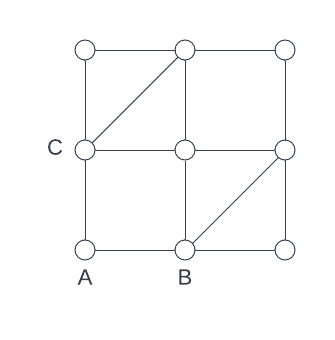
\includegraphics{img/markov-chains/a-b-graph.png}
        \caption{Śmieszny graf \(G\)}
        \label{random_walks:a_b_graph}
    \end{figure}
    \begin{enumerate}[label=(\roman*)]
        \item Wyznacz \(\lim\limits_{n \to \infty} \prob\pars{X_n = A}\) oraz \(\lim\limits_{n \to \infty} \prob\pars{X_n = B}\).
        \item Jaka jest oczekiwana liczba odwiedzeń wierzchołka \(B\) przed pierwszym powrotem do \(A\)?
    \end{enumerate}
\end{exercise}
\begin{proof} Zauważmy, że spacer po naszym grafie \(G\) ma rozkład stacjonarny. Dlaczego? Możemy odhaczyć wszystkie wymagania:
    \begin{itemize}
            \item skończony nieskierowany? --- jak najbardziej
            \item spójny? --- również widać na pierwszy rzut oka
            \item niedwudzielny? --- trójkąty, aż miło patrzeć
    \end{itemize}
    \begin{enumerate}[label=(\roman*)]
        \item Wiemy, że z~własności rozkładu w~skończonym, nieredukowalnym i~ergodycznym łańcuchu Markowa
            \begin{equation*}
                \pi_v = \lim_{t \to \infty} P_{Av}^t = \lim_{t \to \infty} \prob\pars{X_t = v}
            \end{equation*}
            Czyli dokładnie to, czego szukamy. Spacerujemy po grafie, więc
            \begin{equation*}
                \pi_v = \frac{\deg\pars{v}}{2\card{E}}
            \end{equation*}
            Liczymy więc wszystkie krawędzie (jest ich \(14\)) oraz stopnie interesujących nas wierzchołków i~mamy odpowiedź:
            \begin{gather*}
                \lim_{t \to \infty} \prob\pars{X_t = A}
                    = \pi_A
                    = \frac{\deg\pars{A}}{2\card{E}}
                    = \frac{2}{2 \cdot 14}
                    = \frac{1}{14}\\
                \lim_{t \to \infty} \prob\pars{X_t = B}
                    = \pi_B
                    = \frac{\deg\pars{B}}{2\card{E}}
                    = \frac{4}{2 \cdot 14}
                    = \frac{1}{7}
            \end{gather*}
        \item Ułatwimy sobie trochę życie i~policzymy oczekiwaną liczbę odwiedzeń \(B\)~\emph{lub} \(C\) przed pierwszym powrotem do \(A\). Odpowiedź do zadania będzie równa połowie z~tego wyniku, ponieważ sytuacja jest symetryczna.
        
            Zauważmy najpierw, że, będąc w \(B\)~lub \(C\), możemy dojść do \(A\) tylko na jeden sposób --- przechodząc bezpośrednio odpowiednią krawędzią (z~prawdopodobieństwem \(\frac{1}{4}\)). Jest to cenna obserwacja, ponieważ gwarantuje nam, że nie przejdziemy do \(A\) jakąś okrężną drogą. Możemy też być pewni, że natychmiast po wyjściu z~\(A\) znajdziemy się w~\(B\) lub~\(C\) i~dzięki temu pracować pod założeniem, że będziemy w~którymś z~nich przynajmniej raz przed powrotem.
            
            Ponieważ graf jest skończony i~spójny, to wszystkie stany są rekurencyjne. Możemy więc powiedzieć, że mamy rozkład geometryczny z~parametrem \(\frac{1}{4}\): za każdym razem, gdy jesteśmy w~\(B\) lub \(C\) mamy prawdopodobieństwo sukcesu --- powrotu do \(A\) --- równe \(\frac{1}{4}\), a~porażka, ze względu na rekurencyjność, ostatecznie zaprowadzi nas z~powrotem do stanu ,,\(B\) lub \(C\)'' (być może długą drogą, ale w~łańcuchu Markowa trasa, którą obraliśmy, nie ma znaczenia) i~postawi przed takim samym eksperymentem. Zatem tak naprawdę oczekujemy po prostu na sukces, który wypada z~szansą \(\frac{1}{4}\). Oczekiwana liczba prób wynosi zatem \(4\), a~odpowiedź do naszego zadania \(2\).
    \end{enumerate}
\end{proof}
